\documentclass{beamer}
\usepackage[lithuanian]{babel}
\usepackage[utf8x]{inputenc}
\usepackage[L7x]{fontenc}
\usepackage{lmodern}
\usepackage{caption}
\usepackage{subfig}
\usepackage{graphicx}
\usepackage{tikz}
\usetikzlibrary{arrows}

\let\oldshorttitle\insertshorttitle
\renewcommand*\insertshorttitle{
    \leftskip=0.4cm
\oldshorttitle\hfill \insertframenumber\,/\,\inserttotalframenumber
}

\usetheme{Dresden}

\title[Objekto pozicijos nustatymas]{Objekto pozicijos nustatymas naudojant MEMS jutiklius}
\author[M. Norkin]{Maksim Norkin, AKSfm-15}
\institute[VGTU Elektronikos fakultetas]{
    
\includegraphics[height=30px]{img/logo.jpg}\\
    Vilniaus Gedimino technikos universitetas\\
    Elektronikos fakultetas\\
    Elektroninių sistemų katedra\\
    \texttt{maksim.norkin@stud.vgtu.lt}
}

\begin{document}

    \begin{frame}
        \titlepage
    \end{frame}

    \begin{frame}[allowframebreaks]{Jutikliai}
        \begin{itemize}
            \item Pagreičio jutiklis
            \item Giroskopas
            \item Magnetometras
        \end{itemize}

        \framebreak

        \begin{figure}[H]
            \centering
            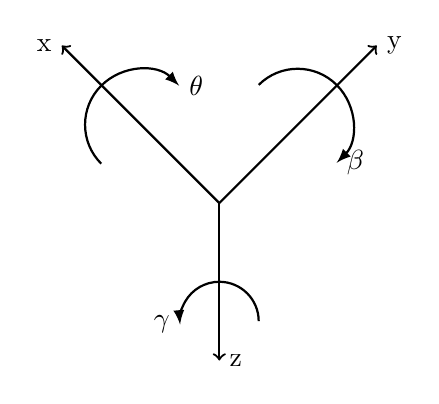
\begin{tikzpicture}
                % axis
                \draw[thick, black, ->] (0,0) -- ( 2, 2) node [right] {y};
                \draw[thick, black, ->] (0,0) -- (-2, 2) node [left] {x}; 
                \draw[thick, black, ->] (0,0) -- ( 0,-2) node [right] {z};
                % arc
                \draw[thick, -latex] ( 0.5,  1.5) arc (135:-45:0.70) node [right] {$\beta$}; 
                \draw[thick, -latex] (-1.5,  0.5) arc (225:45:0.70) node [right] {$\theta$};
                \draw[thick, -latex] ( 0.5, -1.5) arc (0:185:0.5) node [left] {$\gamma$};
            \end{tikzpicture}
            \caption{Objekto pozicijos pagreičio pokyčio ašys, $x$, $y$ ir $z$. Sūkio matmenys apie ašis $\theta$, $\beta$ ir $\gamma$}
            \label{tikz:axis_of_the_system}
        \end{figure}
    \end{frame}

    \begin{frame}{Privalumai \cite{woodman2007introduction}}
        \begin{itemize}
            \item Mažas dydis, svoris
            \item Patvari konstrukcija, patikimi
            \item Salyginai pigu pagaminti
            \item Naudoja mažai galios
        \end{itemize}
    \end{frame}

    \begin{frame}{Trūkumai \cite{woodman2007introduction}}
        Begalės klaidų šaltinių
        \begin{itemize}
            \item Temperatūriniai efektai
            \item Vibraciniai efektai
            \item Kalibravimo klaidos
            \item Nuolatinės dedamosios stabilumas
        \end{itemize}
    \end{frame}

    \begin{frame}[allowframebreaks]{Kalibravimas}
        
        \begin{figure}[H]
            \centering
            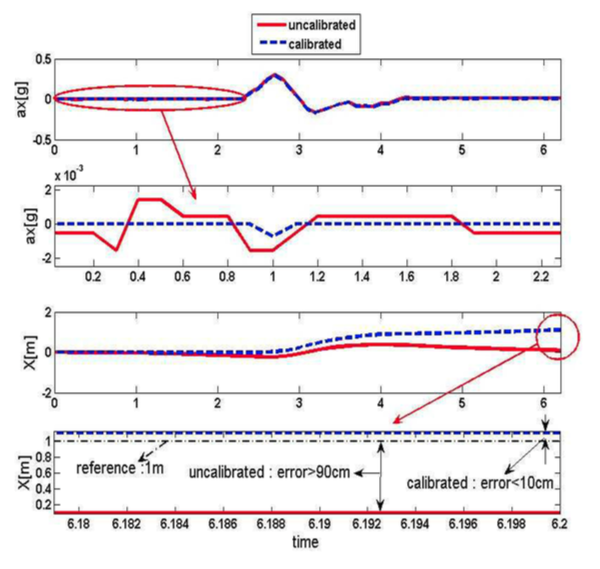
\includegraphics[height=150px]{img/calibration.png}
            \caption{Kalibravimo rezultatas \cite{yoo2011fuzzy}}
        \end{figure}

        \framebreak

        \begin{figure}[H]
            \centering
            \subfloat{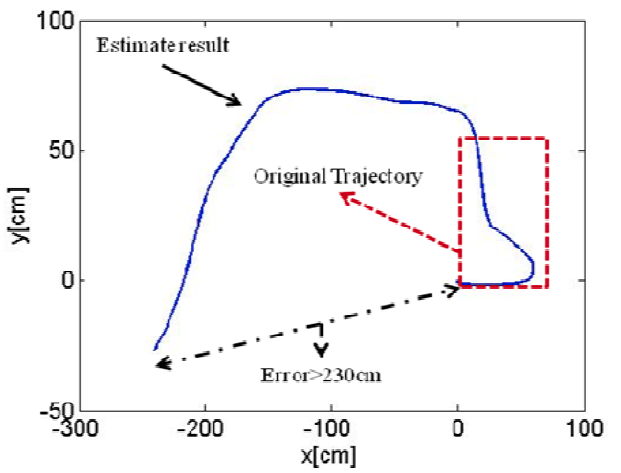
\includegraphics[height=110px]{img/fuzzy_logic_filter_uncalibrated.png}}
            \subfloat{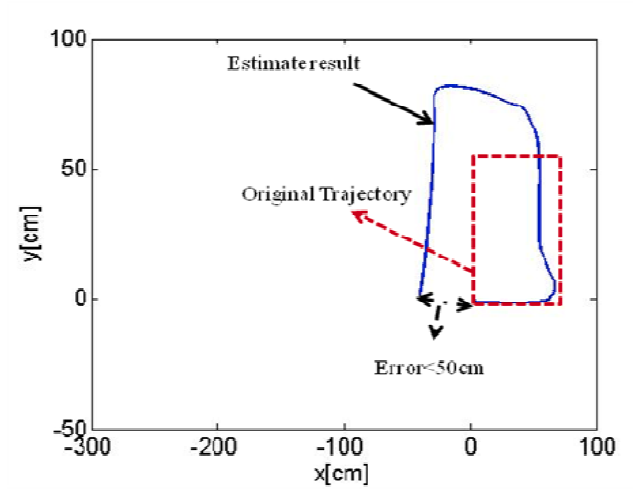
\includegraphics[height=110px]{img/fuzzy_logic_filter_calibrated.png}}
            \caption{Navigacijos rezultatas prieš kalibravimą ir po kalibravimo \cite{yoo2011fuzzy}}
        \end{figure}
    \end{frame}

    \begin{frame}[allowframebreaks]{Filtravimas}

        \begin{figure}[H]
            \centering
            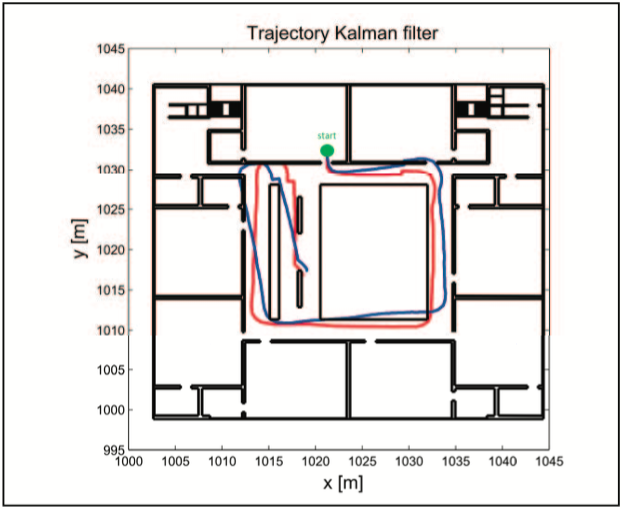
\includegraphics[height=150px]{img/kalman_filter.png}
            \caption{Kalman filtro rezultatas \cite{willemsenconcept}}
        \end{figure}

        \framebreak

        \begin{figure}[H]
            \centering
            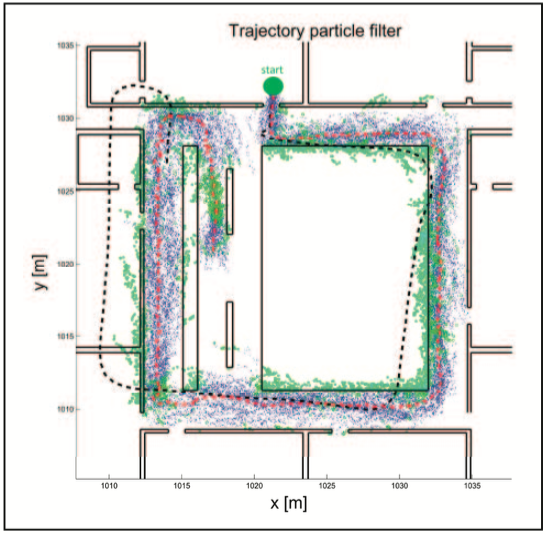
\includegraphics[height=150px]{img/particle_filter.png}
            \caption{Dalelių filtro rezultatas \cite{willemsenconcept}}
        \end{figure}

    \end{frame}

    \begin{frame}{Kitų duomenų pajungimas}
        \begin{figure}
            \centering
            \subfloat{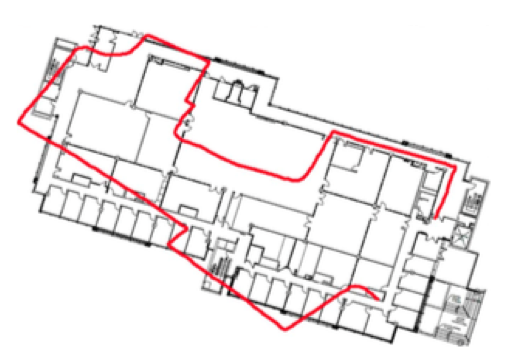
\includegraphics[height=110px]{img/odometer.png}}
            \subfloat{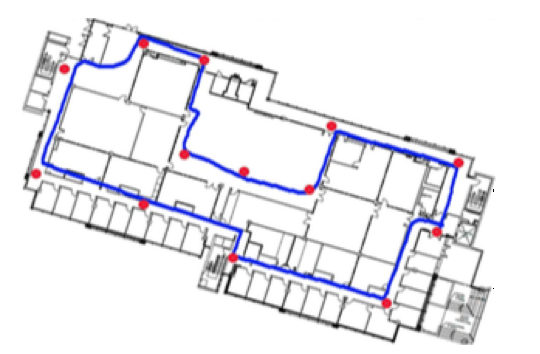
\includegraphics[height=110px]{img/odometer_with_reference.png}}
            \caption{Odometru pagrįsta navigacija be palaikymo ir su palaikymu \cite{atia2015integrated}}
        \end{figure}
    \end{frame}

    \begin{frame}{Išvados}
        \begin{itemize}
            \item Pigu -- reikia naudoti
            \item Spręsti triukšmo problemą
        \end{itemize}
    \end{frame}

    \begin{frame}[allowframebreaks]{Literatūra}
        \bibliographystyle{plain}
        \bibliography{references}

    \end{frame}

\end{document}